\documentclass[tikz]{standalone}
\begin{document}
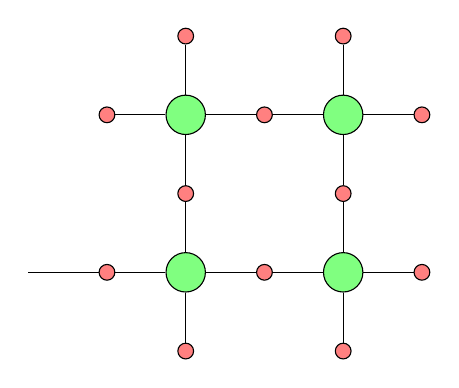
\begin{tikzpicture}
  \tikzstyle{tensor} = [circle, inner sep = 0pt, draw, minimum size = 0.2cm]
  \tikzstyle{Q_tensor} = [tensor, fill=green!50, minimum size = 0.5cm]
  \tikzstyle{delta} = [tensor, fill=red!50, minimum size = 0.2cm]

  % Draw Q tensors
  \foreach \x in {2, 4}
    \foreach \y in {2, 4}
      \node[Q_tensor] (\x-\y) at (\x, \y) {};

  % Draw delta tensors
  \foreach \x in {1, 3, 5}
    \foreach \y in {2, 4}
      {
      \node[delta] (\x-\y) at (\x, \y) {};
      \node[delta] (\y-\x) at (\y, \x) {};
      }

  % Connections
  \foreach \x in {1, ..., 4}
    \foreach \y in {2, 4}
    {
    \pgfmathtruncatemacro{\neighbor}{\x + 1};
    \draw (\x-\y) -- (\neighbor-\y);
    \draw (\y-\x) -- (\y-\neighbor);
    }

  % Outside lines
  \draw (0,2) -- (1-2.west);

\end{tikzpicture}
\end{document}
